\documentclass[a4paper]{article}

\usepackage[spanish]{babel}
\usepackage[utf8]{inputenc}
\usepackage[T1]{fontenc}
\usepackage{float}
\usepackage{graphicx}
\usepackage{amsmath,amssymb,amsfonts}
\usepackage{subcaption}
\usepackage[most]{tcolorbox}
\usepackage{xcolor}
\usepackage[a4paper,top=1cm,bottom=1.5cm,left=3cm,right=3cm,marginparwidth=2.5cm]{geometry}
\usepackage{pgfplots}
\usepackage{palatino}
\pgfplotsset{compat=1.18}
\usetikzlibrary{decorations.pathreplacing,babel}


\newif\ifprintanswers
% \printanswerstrue


\definecolor{miazul}{RGB}{25,43,191}

% Definición de solution con recuadro
\NewEnviron{solution}{%
  \ifprintanswers
    \begin{tcolorbox}[
      colframe=black,     % color del borde
      colback=white,      % fondo blanco
      boxrule=0.8pt,      % grosor de la línea
      arc=0pt,            % esquinas agudas
      left=4pt,           % espacio interior izquierdo
      right=4pt,          % espacio interior derecho
      top=4pt,            % espacio interior superior
      bottom=4pt,         % espacio interior inferior
      before skip=0.5\baselineskip,
      after skip=0.5\baselineskip
    ]
      \textbf{\textit{Respuesta:}}\quad
      \BODY
      \hfill\(\triangleright\)
    \end{tcolorbox}
  \fi
}

\begin{document}

\noindent\makebox[\textwidth]{%
  \texttt{joamartine@fen.uchile.cl}%
  \hfill%
  Mag\'ister en An\'alisis Econ\'omico
}

\vspace{5mm}

\begin{center}
  {\large \textbf{Finanzas Internacionales, Oto\~no 2026}}\\[4pt]
  {\large \textbf{Ayudant\'ia 2}}
\end{center}

\section*{Comentes}

\begin{enumerate}

    \item[a)] Defina el tipo de cambio nominal (TCN) y el tipo de cambio real (TCR). ¿Qu\'e mide cada uno?
    \begin{solution}
    El TCN indica cu\'antas unidades de moneda nacional se necesitan para obtener una unidad de moneda extranjera. El TCR ajusta el TCN por los precios relativos entre pa\'ises:
    \[
    TCR = TCN \cdot \frac{P^*}{P},
    \]
    con \(P^*\) el nivel de precios externo y \(P\) el interno. Mientras el TCN es un precio puramente monetario, el TCR mide el poder adquisitivo relativo y la competitividad de los bienes nacionales frente a los extranjeros.
    \end{solution}

    \item[b)] ¿Cu\'ando se aprecia el TCR y qu\'e implica para la competitividad? Identifique los canales.
    \begin{solution}
    El TCR se aprecia cuando cae (con esta convenci\'on, un TCR menor significa que el pa\'is se vuelve relativamente m\'as caro). De la definici\'on \(TCR = TCN \cdot P^*/P\), esto ocurre por tres canales:
    \begin{itemize}
        \item Apreciaci\'on nominal (cae el TCN).
        \item Aumento de los precios internos \(P\).
        \item Ca\'ida de los precios externos \(P^*\).
    \end{itemize}
    Por ejemplo, si el TCN se mantiene constante pero \(P\) sube m\'as r\'apido que \(P^*\), el cociente \(P^*/P\) cae y el TCR se aprecia. En todos los casos los bienes nacionales se encarecen en t\'erminos relativos, lo que implica una p\'erdida de competitividad externa.
    \end{solution}

    \item[c)] ¿Por qu\'e una depreciaci\'on del TCR tiende a mejorar la balanza comercial?
    \begin{solution}
    Al depreciarse el TCR los bienes nacionales se abaratan para los extranjeros y los bienes extranjeros se encarecen para los nacionales. Esto incentiva las exportaciones y desincentiva las importaciones, mejorando el saldo comercial.
    \end{solution}

    \item[d)] El siguiente gr\'afico muestra la tasa de pol\'itica monetaria (TPM) de Chile y de EE.UU.\ desde 2000. Un analista afirma: ``Como el Banco Central de Chile ha mantenido su tasa en promedio unos 2 puntos por encima de la Reserva Federal, invertir en pesos ha sido sistem\'aticamente m\'as rentable que invertir en d\'olares''. Comente la afirmaci\'on a la luz de la paridad descubierta de tasas y de su relaci\'on con el tipo de cambio.
    \begin{center}
        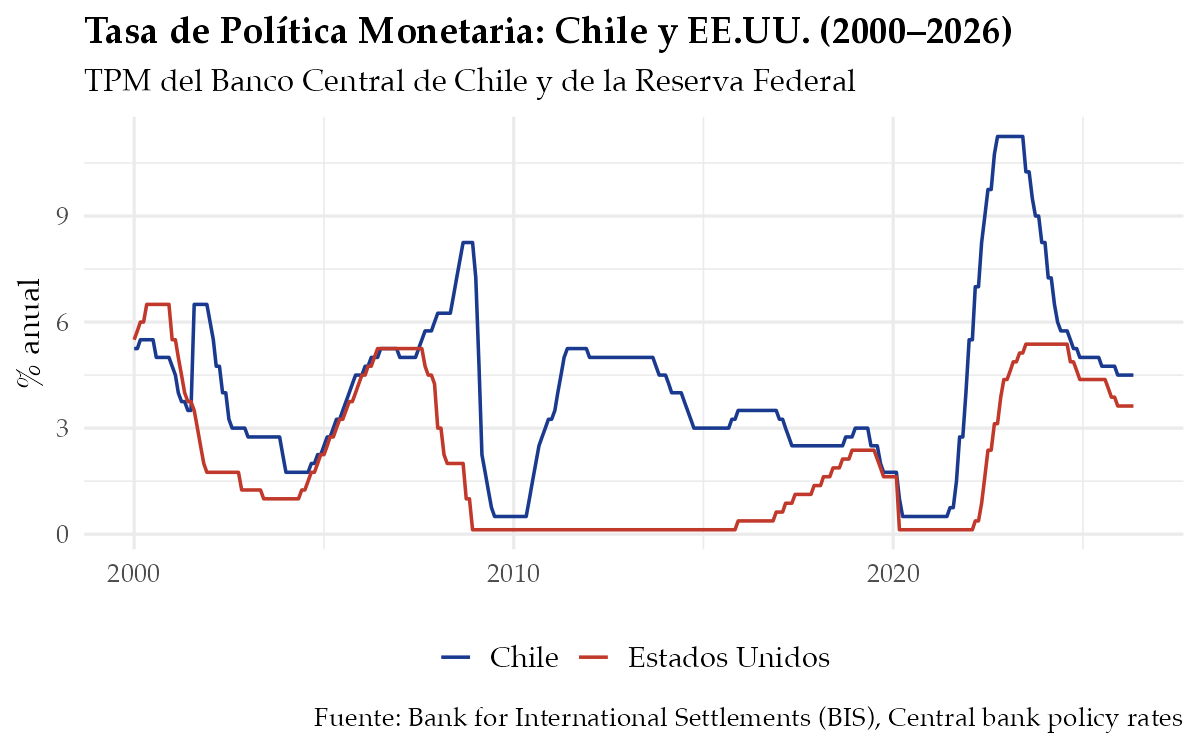
\includegraphics[width=10cm]{tpm_rcode/outputs/tpm_chile_eeuu.png}
    \end{center}
    \begin{solution}
    La afirmaci\'on confunde una mayor tasa nominal con un mayor retorno. La paridad descubierta establece
    \[
    i_t = i_t^* + \frac{e_{t+1}^e - e_t}{e_t} + \rho.
    \]
    Un diferencial persistentemente positivo (en el gr\'afico, del orden de 2 pp en promedio durante 2000--2026) no es una oportunidad de arbitraje, sino la compensaci\'on que el mercado exige por dos factores: la depreciaci\'on esperada del peso y el premio por riesgo pa\'is \(\rho\). En equilibrio, la mayor tasa chilena coexiste con la expectativa de que el peso pierda valor.

    Los datos lo confirman. El siguiente gr\'afico contrasta el diferencial de tasas con la depreciaci\'on interanual efectiva del peso (variaci\'on del tipo de cambio CLP/US\$ a 12 meses). La depreciaci\'on es mucho m\'as vol\'atil que el diferencial y, en promedio, lo supera: durante 2000--2026 el peso se deprecia cerca de un 2,9\% anual frente a un diferencial medio de unos 2,1 pp. Es decir, el peso pierde valor en promedio algo m\'as de lo que rinde el mayor inter\'es local, de modo que el carry hacia el peso result\'o, en promedio, perdedor en el per\'iodo.

    \begin{center}
        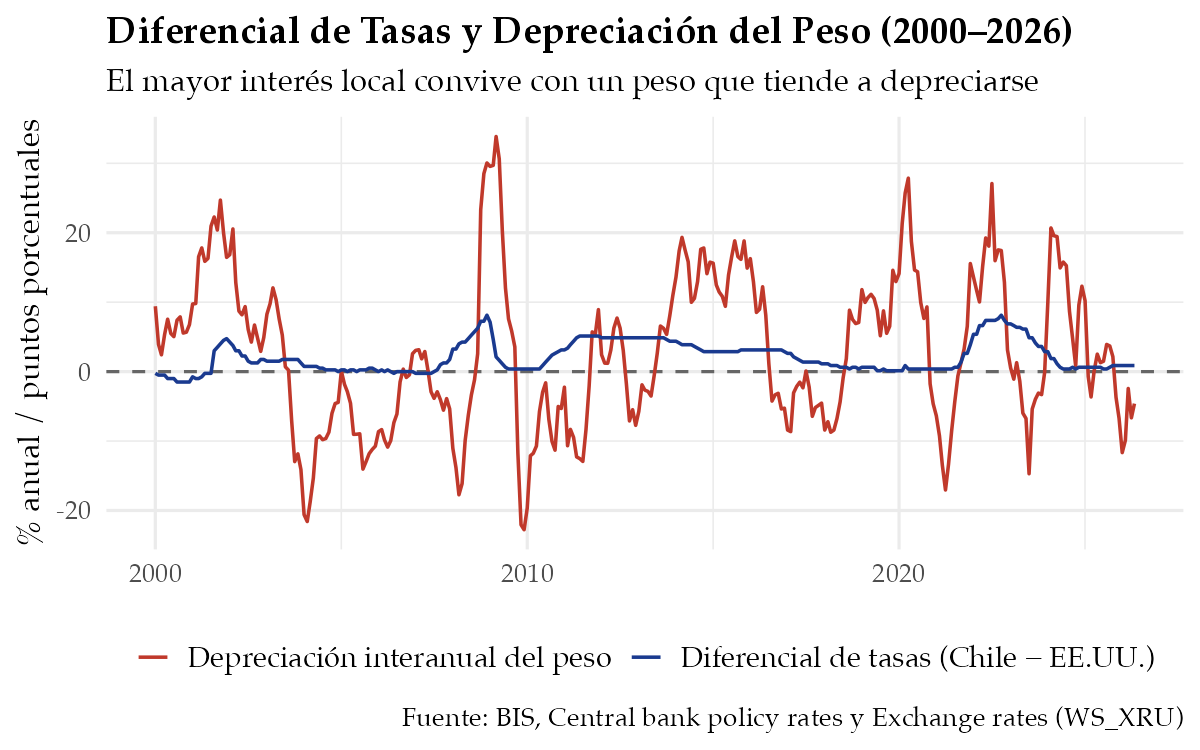
\includegraphics[width=10cm]{tpm_rcode/outputs/diferencial_vs_depreciacion.png}
    \end{center}

    Esto es el ejercicio de carry trade del Matem\'atico II llevado a los datos: solo si la depreciaci\'on efectiva resultara menor que el diferencial neto de riesgo \( (i_t - i_t^* - \rho) \) el carry hacia el peso ser\'ia ganador \emph{ex post}, lo que el gr\'afico muestra que no est\'a garantizado.

    En suma, la afirmaci\'on es incorrecta, bajo la UIP un diferencial de tasas no implica retornos en exceso, sino que anticipa el ajuste del tipo de cambio. El mecanismo conecta con los comentes anteriores: la depreciaci\'on nominal del peso eleva el TCN y, seg\'un el diferencial de inflaci\'on con EE.UU., se traspasa total o parcialmente al TCR.
    \end{solution}

\end{enumerate}

\section*{Matem\'atico I}

Considere una econom\'ia donde la inversi\'on y el ahorro vienen dados por:
\begin{align}
    I &= 100 - 2i  \\
    S &= 50 + 3i
\end{align}
donde $i$ es la tasa de inter\'es (real y nominal son iguales, no hay inflaci\'on).

\begin{itemize}
    \item[a)] Considere una econom\'ia financieramente cerrada. Calcule la tasa de inter\'es de equilibrio y el nivel de ahorro e inversi\'on.

    \begin{solution}
        Igualando $S = I$ se llega a $i = 10$ y $S = I = 80$.

        \begin{center}
        \begin{tikzpicture}[>=latex,xscale=0.14,yscale=0.45]
          \draw[->] (45,0) -- (104,0) node[right] {$S,I$};
          \draw[->] (45,0) -- (45,12) node[above] {$i$};
          \draw[teal,thick] (50,0) -- (86,12) node[above right,teal] {$S(i)$};
          \draw[teal,thick] (100,0) -- (76,12) node[above left,teal] {$I(i)$};
          \draw[dashed] (45,10) -- (80,10);
          \draw[dashed] (80,0) -- (80,10);
          \node[left] at (45,10) {\small $10$};
          \node[below] at (80,0) {\small $80$};
          \fill (80,10) circle (2pt);
        \end{tikzpicture}
        \end{center}
    \end{solution}

    \item[b)] Suponga ahora que la econom\'ia enfrenta una tasa de inter\'es internacional igual a 4 (en porcentajes). Calcule el ahorro dom\'estico $S$, la inversi\'on y el d\'eficit en cuenta corriente. ¿Es esta econom\'ia deudora o acreedora respecto del resto del mundo?

    \begin{solution}
        Dado \( i = 4 \):
        \[
        S = 50 + 3 \cdot 4 = 62, \qquad I = 100 - 2 \cdot 4 = 92.
        \]
        Por lo tanto:
        \[
        CC = S - I = 62 - 92 = -30.
        \]
        Hay un d\'eficit en cuenta corriente de \( -CC = 30 \): la econom\'ia se endeuda con el resto del mundo. Es coherente con que la tasa internacional sea menor que la de autarqu\'ia, reflejando una escasez relativa de recursos internos.

        \begin{center}
        \begin{tikzpicture}[>=latex,xscale=0.14,yscale=0.45]
          \draw[->] (45,0) -- (104,0) node[right] {$S,I$};
          \draw[->] (45,0) -- (45,12) node[above] {$i$};
          \draw[teal,thick] (50,0) -- (86,12) node[above right,teal] {$S(i)$};
          \draw[teal,thick] (100,0) -- (76,12) node[above left,teal] {$I(i)$};
          \draw[dashed,gray] (45,10) -- (80,10);
          \node[left,gray] at (45,10) {\small $10$};
          \draw[dashed] (45,4) -- (92,4);
          \node[left] at (45,4) {\small $4$};
          \draw[dashed] (62,0) -- (62,4);
          \draw[dashed] (92,0) -- (92,4);
          \node[below] at (62,0) {\small $62$};
          \node[below] at (80,0) {\small $80$};
          \node[below] at (92,0) {\small $92$};
          \draw[decorate,decoration={brace,amplitude=4pt,mirror}] (62,2) -- (92,2);
          \node at (77,1) {\small $-CC=30$};
        \end{tikzpicture}
        \end{center}
    \end{solution}

    \item[c)] Suponga ahora movilidad imperfecta de capitales, con oferta de fondos
    \[
        i = 4 - 0{,}2\,CC,
    \]
    donde $-CC$ es el d\'eficit en cuenta corriente. Calcule la tasa de inter\'es de equilibrio, el d\'eficit en cuenta corriente, el ahorro y la inversi\'on.

    \begin{solution}
        En equilibrio \( I = -CC + S \). Con \( i = 4 - 0{,}2\,CC \Rightarrow CC = (4-i)/0{,}2 \), sustituimos:
        \[
        100 - 2i = -\frac{4 - i}{0{,}2} + 50 + 3i = (-20 + 5i) + 50 + 3i = 30 + 8i.
        \]
        Entonces \( 70 = 10i \Rightarrow i = 7 \). Reemplazando:
        \[
        CC = \frac{4 - 7}{0{,}2} = -15 \Rightarrow -CC = 15, \qquad S = 50 + 21 = 71, \qquad I = 100 - 14 = 86.
        \]

        \begin{center}
        \begin{tikzpicture}[>=latex,xscale=0.14,yscale=0.45]
          \draw[->] (45,0) -- (110,0) node[right] {$S,I$};
          \draw[->] (45,0) -- (45,12) node[above] {$i$};
          \draw[teal,thick] (50,0) -- (86,12) node[above right,teal] {$S(i)$};
          \draw[teal,thick] (100,0) -- (76,12) node[above left,teal] {$I(i)$};
          \draw[dotted,thick] (74,4) -- (95,11) node[right] {\scriptsize $i=4+0{,}2(I-S)$};
          \draw[dashed] (45,7) -- (86,7);
          \node[left] at (45,7) {\small $7$};
          \draw[dashed] (71,0) -- (71,7);
          \draw[dashed] (86,0) -- (86,7);
          \node[below] at (71,0) {\small $71$};
          \node[below] at (86,0) {\small $86$};
          \draw[decorate,decoration={brace,amplitude=4pt,mirror}] (71,2) -- (86,2);
          \node at (78.5,1) {\small $-CC=15$};
        \end{tikzpicture}
        \end{center}
    \end{solution}

    \item[d)] Suponga ahora que las exportaciones netas son
    \[
        NX = 3q - 45,
    \]
    donde $q$ es el tipo de cambio real y no hay pagos de factores al exterior. Calcule el TCR de equilibrio en los casos (a), (b) y (c). Compare y comente.

    \begin{solution}
        Sin pagos de factores, \( CC = NX = 3q - 45 \Rightarrow q = (CC + 45)/3 \).
        \begin{itemize}
            \item Caso (a): \( CC = 0 \Rightarrow q = 45/3 = 15 \).
            \item Caso (b): \( CC = -30 \Rightarrow q = 15/3 = 5 \).
            \item Caso (c): \( CC = -15 \Rightarrow q = 30/3 = 10 \).
        \end{itemize}
        El TCR es m\'as depreciado en autarqu\'ia, pues debe ser consistente con \( CC = 0 \). Al abrir la cuenta de capitales, \( I - S > 0 \) (entrada de capitales) aprecia el TCR. Con movilidad imperfecta el efecto es intermedio.
    \end{solution}
\end{itemize}

\section*{Matem\'atico II}

Se conocen los valores nominales y precios de bonos a un a\~no en Estados Unidos y Chile, que pagan su valor nominal al vencimiento.

\begin{center}
\begin{tabular}{|c|c|c|c|}
\hline
\textbf{Bonos} & \textbf{Maduraci\'on} & \textbf{Valor Nominal} & \textbf{Precio} \\
\hline
EE.UU. & 1 a\~no & 255 & 250 US\$ \\
Chile & 1 a\~no & 315 & 300 CLP \\
\hline
\end{tabular}
\end{center}

El tipo de cambio es 470 pesos por d\'olar. El riesgo pa\'is es 1\%.

\medskip
\noindent\textbf{Paridad descubierta de tasas de inter\'es (UIP).} Un inversionista con un peso puede seguir dos estrategias durante un a\~no:
\begin{enumerate}
    \item \emph{Invertir en Chile:} obtiene \( (1+i_t) \) pesos al final del per\'iodo.
    \item \emph{Invertir en EE.UU.:} convierte su peso a d\'olares al tipo de cambio actual (\(1/e_t\) d\'olares), invierte a la tasa externa y obtiene \( (1+i_t^*) \) d\'olares, que reconvierte a pesos al tipo de cambio esperado \( e_{t+1}^e \). En pesos recibe \( \dfrac{e_{t+1}^e}{e_t}(1+i_t^*) \).
\end{enumerate}
Si los activos fueran sustitutos perfectos, ambas estrategias deber\'ian rendir lo mismo. Igualando los retornos brutos,
\[
1 + i_t = \frac{e_{t+1}^e}{e_t}\,(1 + i_t^*),
\]
y tomando la aproximaci\'on de primer orden (productos de t\'erminos peque\~nos despreciables), se obtiene la versi\'on lineal de la paridad descubierta, a la que se a\~nade el premio por riesgo pa\'is \(\rho\) que exigen los inversionistas por mantener el activo chileno:
\[
\;i_t = i_t^* + \underbrace{\frac{e_{t+1}^e - e_t}{e_t}}_{\text{depreciaci\'on esperada}} + \rho\;
\]
\textbf{Mecanismo.} La paridad es una condici\'on de no arbitraje. Si el retorno en pesos de un activo supera al del otro, los inversionistas se vuelcan hacia el m\'as rentable: compran ese activo (y su moneda) y venden el otro. Este flujo de capitales presiona los precios, los tipos de cambio (spot y esperado) y las tasas hasta que ambos retornos se igualan. El t\'ermino \( (e_{t+1}^e - e_t)/e_t \) refleja que una depreciaci\'on esperada del peso encarece el retorno en pesos del activo externo, compensando su menor tasa nominal.

\begin{itemize}
    \item[a)] ¿Cu\'al es la tasa de inter\'es del bono en EE.UU.\ y Chile?
    \begin{solution}
        \[
        i_t^* = \frac{255}{250} - 1 = 2{,}0\%, \qquad i_t = \frac{315}{300} - 1 = 5{,}0\%.
        \]
    \end{solution}

    \item[b)] Calcule el tipo de cambio futuro consistente con la paridad de tasas de inter\'es.
    \begin{solution}
        El tipo de cambio futuro de paridad es aquel que iguala el retorno en pesos de ambos bonos. Imponiendo la condici\'on de no arbitraje:
        \[
        i_t = i_t^* + \frac{e_{t+1} - e_t}{e_t} + \rho
        \quad\Rightarrow\quad
        5{,}0\% = 2{,}0\% + \frac{e_{t+1} - 470}{470} + 1{,}0\%.
        \]
        Despejando la depreciaci\'on esperada:
        \[
        \frac{e_{t+1} - 470}{470} = 5{,}0\% - 2{,}0\% - 1{,}0\% = 2{,}0\%
        \quad\Rightarrow\quad
        e_{t+1} = 470 \,(1 + 0{,}02) = 479{,}4.
        \]
        Interpretaci\'on: como el bono chileno paga 3 puntos m\'as que el estadounidense pero exige 1 punto de premio por riesgo, el mercado solo estar\'a indiferente entre ambos si espera que el peso se deprecie un 2\% (el peso debe perder valor para compensar la mayor tasa local). A ese tipo de cambio esperado nadie tiene incentivo a mover capitales y se sostiene el equilibrio.
    \end{solution}

    \item[c)] ¿Qu\'e bono preferir\'an los inversionistas si esperan que el peso se deprecie a \$/US\$ 490 el a\~no siguiente? Demuestre matem\'aticamente.
    \begin{solution}
        Comparamos el retorno en pesos de cada estrategia. Bono de EE.UU.\ (medido en pesos): invertir 250 US\$ cuesta \( 250 \times 470 = 117{,}500 \) CLP y se reciben \( 255 \times 490 = 124{,}950 \) CLP. Rentabilidad:
        \[
        r_{\text{EE.UU.}} = \frac{124{,}950 - 117{,}500}{117{,}500} \approx 6{,}34\%.
        \]
        Bono de Chile:
        \[
        r_{\text{Chile}} = \frac{315 - 300}{300} = 5{,}0\%.
        \]
        Como \( 6{,}34\% > 5{,}0\% \), prefieren el bono de EE.UU.

        \medskip
        El mismo resultado se obtiene con la UIP. El retorno esperado en pesos del activo externo (lado derecho de la paridad) es
        \[
        i_t^* + \frac{e_{t+1}^e - e_t}{e_t} + \rho
        = 2{,}0\% + \frac{490 - 470}{470} + 1{,}0\%
        \approx 2{,}0\% + 4{,}26\% + 1{,}0\% = 7{,}26\%,
        \]
        que supera al retorno del bono chileno \( i_t = 5{,}0\% \). La paridad ya no se cumple: la depreciaci\'on esperada (490) excede a la de equilibrio (479,4), de modo que la ganancia cambiaria m\'as que compensa la menor tasa externa.

        \textbf{Mecanismo de ajuste.} Ante este desequilibrio, los inversionistas venden bonos chilenos y compran d\'olares para invertir en EE.UU. Esta presi\'on de compra de d\'olares hoy tiende a subir el tipo de cambio spot \(e_t\), lo que reduce la depreciaci\'on esperada restante \((e_{t+1}^e - e_t)/e_t\); el proceso contin\'ua hasta que ambos retornos vuelven a igualarse y se restablece la paridad.

        \textbf{Carry trade.} Este es un caso de \emph{carry trade}: endeudarse en la moneda de tasa baja (d\'olar) e invertir en la de tasa alta (peso). El carry neto es \( i_t - i_t^* - \rho = 2\% \), igual a la depreciaci\'on de equilibrio de (b). Como aqu\'i la depreciaci\'on esperada (4,26\%) supera ese 2\%, el carry hacia el peso se espera perdedor y conviene la estrategia inversa: invertir en d\'olares.
    \end{solution}

    \item[d)] Un economista se\~nala que la depreciaci\'on del peso de las \'ultimas semanas tendr\'a efectos inflacionarios en el IPC. ¿Es correcta la aseveraci\'on? Explique.
    \begin{solution}
        Los hogares consumen bienes nacionales e importados, por lo que una depreciaci\'on del peso encarece los importados y se traspasa al IPC en el corto y mediano plazo. La aseveraci\'on es correcta.
    \end{solution}
\end{itemize}

\end{document}